\documentclass[11pt, openright]{book}

    % Cover Variables
    \newcommand{\ctoptitle}{}
    \newcommand{\ctitle}{Title}
    \newcommand{\cautor}{Author}
    \newcommand{\cdate}{day.month.year}
    \newcommand{\sectittle}{Second Title}


    % Header Variables
        \newcommand{\headRE}{Main Topic}
        \newcommand{\headLE}{\emph{\rightmark}}
        \newcommand{\footRE}{Lucas Lescure $-$ \cdate}
        \newcommand{\footLE}{\emph{\thepage}}

    % TOC Variables
        \newcommand{\toctitle}{Table of Content}
        
        \newcommand{\tocchapter}{Chapter}
        \newcommand{\toccount}{3}
  
    % Chapter Variables
        \newcommand{\chvar}{Chapter -}
        
\usepackage[a4paper, total={16cm, 22.125cm}]{geometry}

% Page Style
\usepackage[]{environ}
% Cover Page 
\usepackage{tikz}
\makeatletter
\def\parsecomma#1,#2\endparsecomma{\def\page@x{#1}\def\page@y{#2}}
\tikzdeclarecoordinatesystem{page}{
    \parsecomma#1\endparsecomma
    \pgfpointanchor{current page}{north east}
    % Save the upper right corner
    \pgf@xc=\pgf@x%
    \pgf@yc=\pgf@y%
    % save the lower left corner
    \pgfpointanchor{current page}{south west}
    \pgf@xb=\pgf@x%
    \pgf@yb=\pgf@y%
    % Transform to the correct placement
    \pgfmathparse{(\pgf@xc-\pgf@xb)/2.*\page@x+(\pgf@xc+\pgf@xb)/2.}
    \expandafter\pgf@x\expandafter=\pgfmathresult pt
    \pgfmathparse{(\pgf@yc-\pgf@yb)/2.*\page@y+(\pgf@yc+\pgf@yb)/2.}
    \expandafter\pgf@y\expandafter=\pgfmathresult pt
}
\makeatother


% Object formatting
\usepackage[12pt]{moresize}
\usepackage[]{anyfontsize}
\usepackage{titlesec}
\usepackage{import}
\usepackage{floatrow}
\usepackage{enumitem}
\usepackage{changepage}
\usepackage[normalem]{ulem}
\usepackage{array}
\newcommand{\ul}[1]{\underline{#1}}

\usepackage[]{chngcntr}
\usepackage{ifthen}
\ifthenelse{\figcountdepth > 1}
  {\counterwithin{figure}{section}\counterwithin{table}{section}}
  {}

\usepackage[format=plain, labelfont=it, textfont=it]{caption}
\makeatletter
\def\@makecaption#1#2{%
    \vskip\abovecaptionskip
    \sbox\@tempboxa{\textit{#1.} #2}

       
   

    \ifdim \wd\@tempboxa >\hsize
        #1. #2\par
    \else
        \global \@minipagefalse
        \hb@xt@\hsize{\hfil\box\@tempboxa\hfil}
    \fi
    \vskip\belowcaptionskip}
\makeatother

\DeclareCaptionFormat{underline}{\uline{#1#2#3}\par}

% Sections
\titleformat{\section}{\fontsize{16}{19.2}\bfseries}{\thesection.}{0.25em}{}
\titleformat{\subsection}{\fontsize{14}{16.8}\bfseries}{\tab\thesubsection.}{0.25em}{}
\titleformat{\subsubsection}{\fontsize{10}{12}}{\uline{\thesubsubsection)\enspace}}{0em}{\uline}





% Geometry

% Typewritting

\setlength{\parskip}{1em}
\setlength{\parindent}{0em}


\newenvironment{items}[3][0pt]
{\def\closesep{#3}
    \vspace{#2}
    \begin{itemize}
        \setlength{\itemsep}{#1}
        \setlength{\topsep}{0pt}
        \setlength{\partopsep}{0pt}}
        {\end{itemize}
    \vspace{\closesep}}

\newenvironment{enum}[3][0pt]
{\defclosesep{#3}
    \vspace{#2}
    \begin{enumerate}
        \setlength{\itemsep}{#1}
        \setlength{\topsep}{0pt}
        \setlength{\partopsep}{0pt}}
        {\end{enumerate}
    \vspace{\closesep}}

\newenvironment{eq}[2]
{\def\closesep{#2}
    \vspace{#1}
    \begin{align*}}
        {\end{align*}
    \vspace{\closesep}}

\newenvironment{lfeq}[2]
{\def\closesep{#2}
    \vspace{#1}
    \begin{flalign*}}
        {\end{flalign*}
    \vspace{\closesep}}
% List Formatting


\NewEnviron{dent}[1]{
    \vspace{-10pt}
    \begin{adjustwidth}{7mm}{}
        \uline{#1}\hspace{2mm}
        \BODY
    \end{adjustwidth}
    \vspace{-10pt}
}


\usepackage[framemethod=tikz]{mdframed}
\newcounter{count_theorem}[section]\setcounter{count_theorem}{0}
\newcommand{\thetheorem}{\arabic{count_theorem}}

\newcounter{count_exercise}[section]\setcounter{count_exercise}{0}
\newcommand{\theexercise}{\arabic{count_exercise}}


\newenvironment{theorem}[1][]{
    \refstepcounter{count_theorem}
    \mdfsetup{
        linecolor=red!30,
        innerbottommargin=10pt,
        linewidth=2pt,
        topline=false,
        bottomline=false,
        rightline=false,
        shadow=true,
        shadowsize=4.5pt,
        frametitlerule=false,
        apptotikzsetting={
                \tikzset{
                    mdfbackground/.append style={
                            left color=red!8,right color=red!3
                        }
                }
            }
    }
    \begin{mdframed}[]\relax
        \ifstrempty{#1}
        {\textbf{Theorem~\thetheorem.} }
        {\textbf{Theorem~\thetheorem.~#1} }
        }
        {\end{mdframed}\vspace{-10pt}
}

\newenvironment{note}{
    \mdfsetup{innertopmargin=5pt,
        linecolor=gray!30,
        linewidth=2pt,
        topline=false,
        bottomline=false,
        rightline=false,
        frametitleaboveskip=0pt,
        shadow=false,
        shadowsize=4pt,
        frametitlerule=false,
        apptotikzsetting={
                \tikzset{
                    mdfbackground/.append style={
                            left color=gray!8,right color=gray!3
                        }
                }
            }
    }
    \begin{mdframed}[]\relax
        \textbf{Note. }
        }
        {\end{mdframed}\vspace{-10pt}
}

\newenvironment{example}{
    \mdfsetup{innertopmargin=5pt,
        linecolor=green!30,
        linewidth=2pt,
        topline=false,
        bottomline=false,
        rightline=false,
        frametitleaboveskip=0pt,
        shadow=false,
        shadowsize=4pt,
        frametitlerule=false,
        apptotikzsetting={
                \tikzset{
                    mdfbackground/.append style={
                            left color=green!7,right color=green!2
                        },
                    mdfframetitlebackground/.append style={
                            left color=green!7,right color=green!2
                        }
                }
            }
    }
    \begin{mdframed}[]\relax
        \textbf{Example. }
        }
        {\end{mdframed}\vspace{-10pt}
}


\usetikzlibrary{calc,arrows}

\tikzset{
    excursus arrow/.style={%
            line width=2pt,
            draw=gray!40,
            rounded corners=2ex,
        },
    excursus head/.style={
            fill=white,
            font=\bfseries\sffamily,
            text=gray!80,
            anchor=base west,
        },
    excursus line/.style={%
            line width=2pt,
            draw=gray!40,
            rounded corners=2ex,
        }
}

\newenvironment{exercise}[1][]{%
    \refstepcounter{count_exercise}
    \mdfsetup{
        singleextra={
                \path let \p1=(P), \p2=(O) in (\x2,\y1) coordinate (Q);
                \path let \p1=(Q), \p2=(O) in (\x1,{(\y1-\y2)/2}) coordinate (M);
                \path [excursus line] ($(O)+(5em,0ex)$) -| (M) |- ($(Q)+(20em,0ex)$);
                \node [excursus head] at ($(Q)+(2.5em,-0.75pt)$) {\ifstrempty{#1}{Exercise \theexercise}{Exercise \theexercise:~#1}};},
        firstextra={
                \path let \p1=(P), \p2=(O) in (\x2,\y1) coordinate (Q);
                \path [excursus arrow,-to] (O) |- ($(Q)+(12em,0ex)$) .. controls +(0:16em) and +(185:6em) .. ++(23em,2ex);},
        middlelinewidth=2.5em,middlelinecolor=white,
        hidealllines=true,topline=true,
        innertopmargin=0.5ex,
        innerbottommargin=2.5ex,
        innerrightmargin=2pt,
        innerleftmargin=2ex,
        skipabove=0.87\baselineskip,
        skipbelow=0.62\baselineskip,
    }
    \begin{mdframed}[]\relax}
        {\end{mdframed}\vspace{-10pt}
}

% Functions and Data Plotting
\usepackage{subfig,wrapfig,adjustbox,multirow}


% Plotting Style
\usepackage{graphicx,pgfplots}
\usetikzlibrary{arrows}
\usetikzlibrary {patterns,patterns.meta}
\usepgfplotslibrary{fillbetween}
\pgfplotsset{compat=1.18}

\usepgfplotslibrary{units}
% Logarithmic Scale
\pgfplotsset{
    log x ticks with fixed point/.style={
            xticklabel={
                    \pgfkeys{/pgf/fpu=true}
                    \pgfmathparse{exp(\tick)}%
                    \pgfmathprintnumber[fixed relative, precision=3]{\pgfmathresult}
                    \pgfkeys{/pgf/fpu=false}
                }
        }
}


% Mathematics

% Formatting
\usepackage{amsmath}
\usepackage{esvect}
\usepackage{amsfonts}
\usepackage{tasks,environ}
\usepackage{xargs}
\usepackage{esint}
\usepackage[]{listings}


\usepackage[english]{babel}
\usepackage{amsthm}
%\newtheorem{theorem}{Theorem}
%\newtheorem{proof}{Proof}



%Custom Shortcuts
\newcommand{\eqi}{\Leftrightarrow}
\newcommand{\lr}[1]{\left( #1 \right)}
\newcommand{\limit}[1]{\displaystyle{\lim_{#1}}}
\newcommand{\tab}{\hspace*{7mm}}
\newcommand{\ds}[1]{\displaystyle{#1}}
\newcommand{\floor}[1]{\lfloor #1 \rfloor}
\newcommand{\R}{\mathbb{R}}
\newcommand{\N}{\mathbb{N}}
\newcommand{\Z}{\mathbb{Z}}
\newcommand{\C}{\mathbb{C}}
\newcommand{\K}{\mathbb{K}}
\newcommand{\F}{\mathcal{F}}
\newcommand{\M}{\mathcal{M}}
\renewcommand{\l}{\lambda}
\newcommand{\seg}[1]{\overline{\rm {#1}}}
\newcommand{\Int}{\int\limits}
\newcommand{\ex}{\tab \uline{Example :}\hspace{0.2cm} }
\newcommand{\vard}{\partial}
\newcommand{\Q}{\mathcal{Q}}
\newcommand{\Vect}{\operatorname{Vect}}
\newcommand{\rg}{\operatorname{rg}}
\renewcommand{\dim}{\operatorname{dim}}
\renewcommand{\Re}{\operatorname{Re}}
\renewcommand{\Im}{\operatorname{Im}}
\renewcommand{\P}{\mathcal{P}}
\newcommand{\blr}[1]{\left\{#1\right\}}
\newcommand{\linecenter}[1]{\par\vspace{2mm} \centerline{#1}\par\vspace{-2mm}}
\newcommand{\dd}{\textrm{d}}
\newcommand{\supp}{\operatorname{Supp}}
\renewcommand{\vec}{\overrightarrow}
\renewcommand{\epsilon}{\varepsilon}

% Matrix Configurations

\makeatletter
\renewcommand*\env@matrix[1][*\c@MaxMatrixCols c]{%
    \hskip -\arraycolsep
    \let\@ifnextchar\new@ifnextchar
    \array{#1}}
\makeatother


% Colors
\usepackage{xcolor}
\newcommand{\blu}{\color{blue}}
\newcommand{\Red}{\color{red}}
\newcommand{\blac}{\color{black}}

\newcommand{\red}[1]{\textcolor{red}{#1}}

\usepackage{xcolor,xspace}
\usepackage{breqn}


% Headings  
\usepackage[Glenn]{fncychap}
\ChNumVar{\fontsize{40}{42}}
\ChTitleVar{\Large\sc}
\ChNameVar{\Large\sc}
\setlength\headheight{14.5pt}
\renewcommand\FmN[1]{\chvar}



\usepackage{fancyhdr}
\usepackage{ragged2e}

% Header & Footers
\renewcommand{\chaptermark}[1]{\markboth{#1}{#1}}
\renewcommand{\sectionmark}[1]{
    \markright{ #1}
}
\pagestyle{fancy}
\fancyhf{}
\fancyhead[LE,RO]{\headLE}
\fancyhead[RE,LO]{\headRE}
\fancyfoot[LE,RO]{\footLE}
\fancyfoot[RE,LO]{\footRE}
\renewcommand{\headrulewidth}{0.5pt}
\fancyheadoffset{1cm}

\fancypagestyle{plain}{%
    \fancyhf{} % clear all header and footer fields
    \fancyfoot[LE, RO]{\footLE}
    \renewcommand{\headrulewidth}{0pt}
    \renewcommand{\footrulewidth}{0pt}}


\fancypagestyle{nohead}{%
    \fancyhf{} % clear all header 
    \fancyfoot[LE, RO]{\footLE}
    \fancyfoot[LO, RE]{\footRE}}

    \fancypagestyle{head}{%
    \fancyhf{} % clear all header 
    \fancyhead[LE,RO]{\headLE}
\fancyhead[RE,LO]{\headRE}
\renewcommand{\headrulewidth}{0.5pt}
\fancyheadoffset{1cm}
    }


\fancypagestyle{bib}{%
    \fancyhf{} % clear all header and footer fields
    \fancyhead[CE, CO]{}
    \fancyfoot[LE, RO]{\footLE}
    \fancyfoot[LO, RE]{Bibliographie}}

% Table of Contents

\renewcommand*\thechapter{\arabic{chapter}} %Usually Roman
\renewcommand*\thesection{\arabic{section}}
\renewcommand*\thesubsubsection{\thesubsection.\alph{subsubsection}}
\makeatletter
\@removefromreset{section}{chapter}
\makeatother


% Table of Contents

\usepackage{titletoc}
\usepackage{ erewhon,cabin}
\usepackage[linktoc=all]{hyperref}
\renewcommand*\contentsname{\centerline{\toctitle}}

\setcounter{secnumdepth}{3}
\setcounter{tocdepth}{\toccount}

\usepackage[subfigure]{tocloft}
\setlength\cftparskip{0pt}

\usepackage{etoolbox}
\makeatletter
\pretocmd{\chapter}{\addtocontents{toc}{\protect\addvspace{5\p@}}}{}{}
\pretocmd{\section}{\addtocontents{toc}{\protect\addvspace{-10\p@}}}{}{}
\pretocmd{\subsection}{\addtocontents{toc}{\protect\addvspace{1\p@}}}{}{}
\makeatother


% Chapter Style
\titlecontents{chapter}
[11em]
{\bigskip}
{\bfseries\textsc\tocchapter~\textsc\thecontentslabel : \textsc}
{\hspace*{-5.5em}\textbf}
{\titlerule*[1pc]{ }}[\smallskip]

% Section Style
\titlecontents{section}
[0em] % i
{\bigskip\bfseries}
{\fontsize{11}{13.2}\bfseries\uline{\thecontentslabel.\enspace}\uline}
{\hspace*{-4em}\textbf}
{\hspace{0.5pt}\uline{\hspace*{\fill}}\contentspage}

% Subsection Style
\titlecontents{subsection}
[2em] % i
{\smallskip\bfseries}
{\fontsize{10}{12}\bfseries\thecontentslabel.\enspace}
{\hspace*{-4em}}
{\titlerule*[0.5pc]{.}\contentspage}

% Subsubsection Style
\titlecontents{subsubsection}
[4em] % i
{\smallskip}
{\fontsize{10}{12}\thecontentslabel)\enspace}
{\hspace*{-4em}}
{\titlerule*[0.5pc]{.}\contentspage}










    % figure support
    \usepackage{import}
    \usepackage{xifthen}
    \pdfminorversion=7
    \usepackage{pdfpages}
    \usepackage{transparent}
    \newcommand{\incfig}[1]{%
            \def\svgwidth{\columnwidth}
            \import{./figures/}{#1.pdf_tex}
    }

    \pdfsuppresswarningpagegroup=1

\usepackage{lipsum}
    
    

\begin{document}
% Spacing
% Section Spacing
\titlespacing\section{0pt}{3pt plus 2pt minus 2pt}{6pt plus 2pt minus 1pt}
\titlespacing\subsection{0pt}{0pt plus 1pt minus 1pt}{0pt plus 3pt minus 1pt}
\titlespacing\subsubsection{0pt}{0pt plus 0pt minus 0pt}{0pt plus 2pt minus 0pt}

\usetikzlibrary{shadows}

\newgeometry{left=2.5cm, width=16cm, bottom=2.5cm, top=2.5cm}






% Cover
% Cover
\definecolor{ccolor1}{RGB}{236,145,143}
\definecolor{ccolor2}{RGB}{131,168,192}
\definecolor{ccolor3}{RGB}{182,227,150}
\definecolor{ccolor4}{RGB}{171,206,145}

\usetikzlibrary{fadings}

\begin{titlepage}
    \newgeometry{top=1cm, width=21cm, bottom=1cm}

    \begin{tikzpicture}[remember picture,overlay,every node/.style={anchor=center}]

        \coordinate (Center) at (page cs: 0,-0.5);
        %F4E Logo
        \begin{scope}[scale = 1.5]
            \foreach \angle in {0,30,...,330} {
                    \filldraw[orange!50!yellow,line width=0.01pt,shift=(Center)] (\angle:3.8637) -- (\angle+30:3.8637) -- (0,0) -- (\angle:3.8637);
                    \draw[white, line width = 7pt,shift=(Center)] (\angle:2cm) arc (\angle-60:\angle:2cm);
                    \draw[white, line width = 7pt,shift=(Center)] (\angle+30:2cm) arc (\angle+90:\angle+30:2cm);
                }
            % Outer delimiter
            \foreach \angle in {15,45,...,345} {
                    \filldraw[white, line width = 7pt,shift=(Center)] (\angle:3.8637cm) arc (\angle-15:\angle+45:2cm) arc (\angle+15:\angle-15:2cm) arc (\angle+45:\angle+15:2cm);
                }
            % Inner delimiter
            \foreach \angle in {15,45,...,345} {
                    \filldraw[white, line width = 7pt,shift=(Center)] (\angle:1.0353cm) arc (\angle-75:\angle-45:2cm) arc (\angle+75:\angle+105:2cm) -- (0,0) -- (\angle:1.0353cm);
                }
            % Stars
            \foreach \angle in {0,30,...,330} {
                    \fill[orange!50!yellow,shift=(Center)] (\angle:1.03527cm) -- ++ (231:0.175) -- ++ (33:0.35) -- ++ (177:0.35) -- ++ (321:0.35) -- ++ (105:0.35) -- ++ (249:0.35) -- ++ (33:0.35);
                }
        \end{scope}

        \node[opacity =0.07, inner sep=0pt, anchor=east] at (current page.east){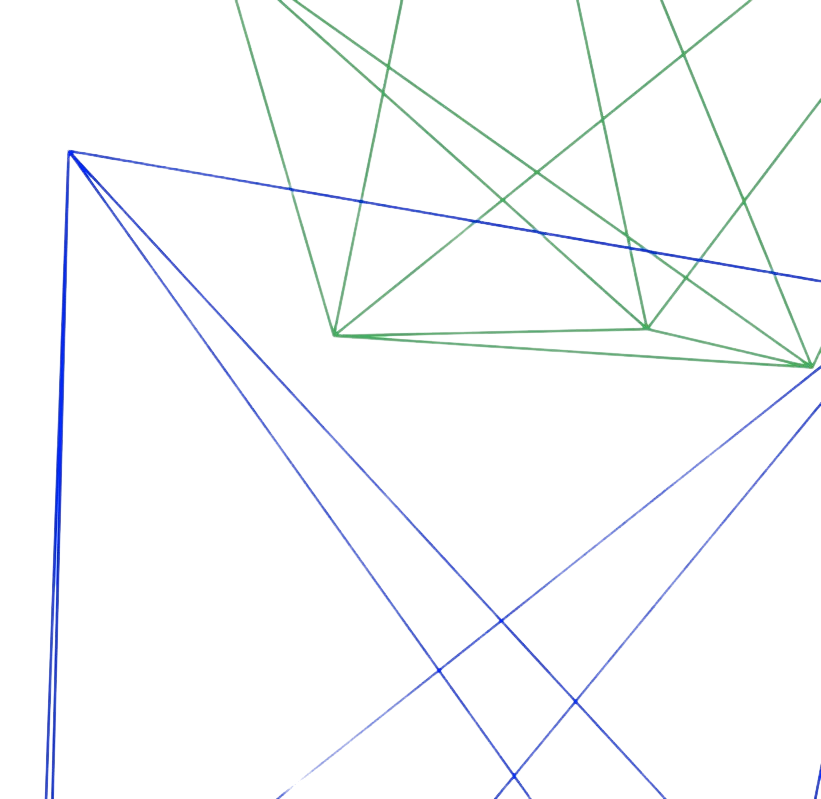
\includegraphics[width=0.5\paperwidth,height=\paperheight]{/root/.config/latex-utils/logos/invert1.png}};

        \node[opacity=0.07,inner sep=0pt, anchor=north west] at (current page.north west){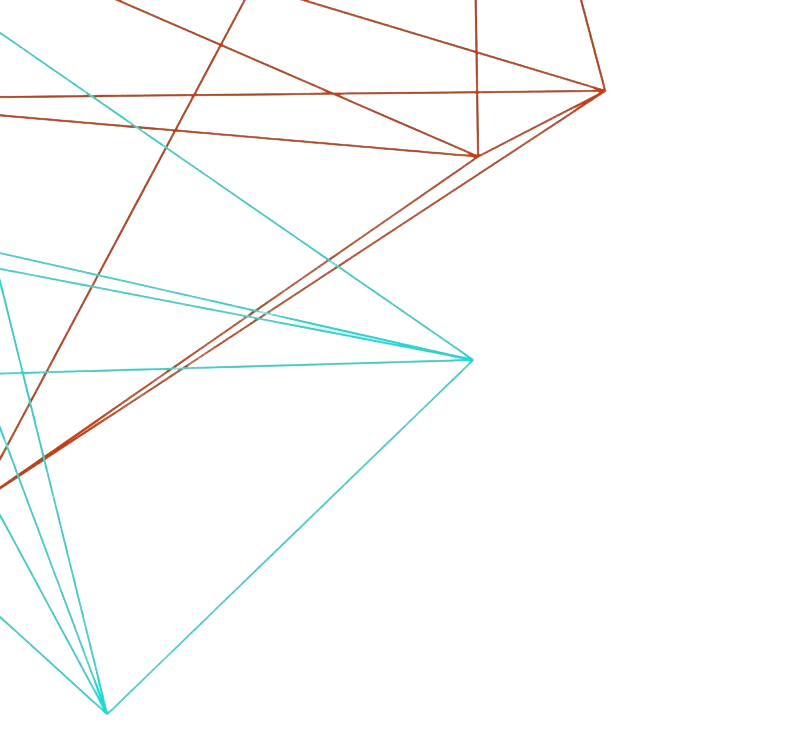
\includegraphics[width=0.5\paperwidth,height=0.5\paperheight]{/root/.config/latex-utils/logos/invert3.png}};




        \node at (page cs:0,0.345) {\Large\textsc{High School Observation and Learning Internship}};
        \node at (page cs:0,0.875) {\Large\bfseries\textsc{Observation Internship}};
        \node at (page cs:0,0.925) {\LARGE\bfseries\textsc{Lycée Français de Barcelone}};

        \node at (page cs:0.5,0) {\Large\textsc{Cyril Lescure - Pedagogical Tutor}};








        %\node[opacity=0.15, inner sep=0pt, anchor=south west] at (current page.south west){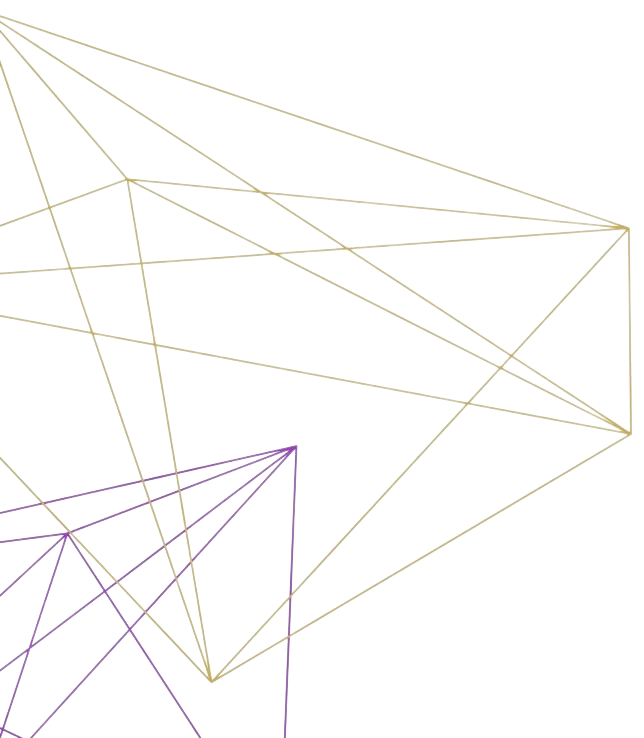
\includegraphics[width=0.5\paperwidth,height=0.5\paperheight]{/root/.config/latex-utils/logos/invert2.png}};

        \node at (page cs:0,0.5) {\fontsize{28}{28.8}\textbf{\ctoptitle}};
        \node at (page cs:0,0.425) {\fontsize{28}{28.8}\textbf{\ctitle}};
        \draw (page cs:0.5,0.375) -- (page cs:-0.5,0.375);
        \node at (page cs:0,0.245) {\LARGE\textsc{\cautor}};
        \node at (page cs:0,0.310) {\Large\textsc{03.06.2019 - 07.06.2019}};


    \end{tikzpicture}
\end{titlepage}


\newgeometry{width=18.625cm, bottom=2cm, top=2cm}

\tikz[remember picture, overlay] \node[opacity=0.3,inner sep=0pt, anchor=north east] at (current page.north east){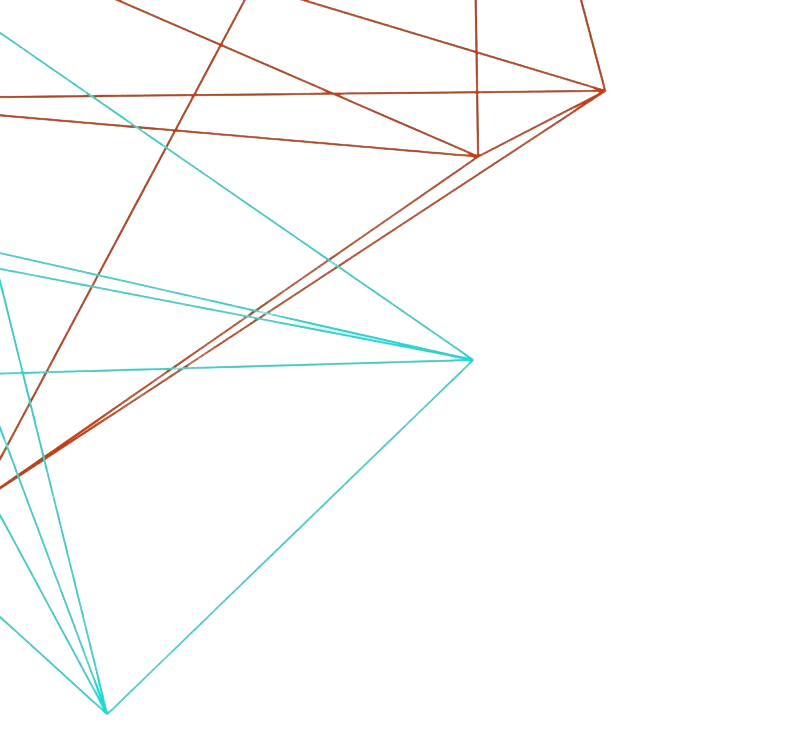
\includegraphics[angle=-90,origin=c,width=0.5\paperheight,height=0.5\paperwidth]{/root/.config/latex-utils/logos/invert3.png}};
\tikz[remember picture,overlay] \node[opacity=0.3,inner sep=0pt, anchor=south east] at (current page.south east){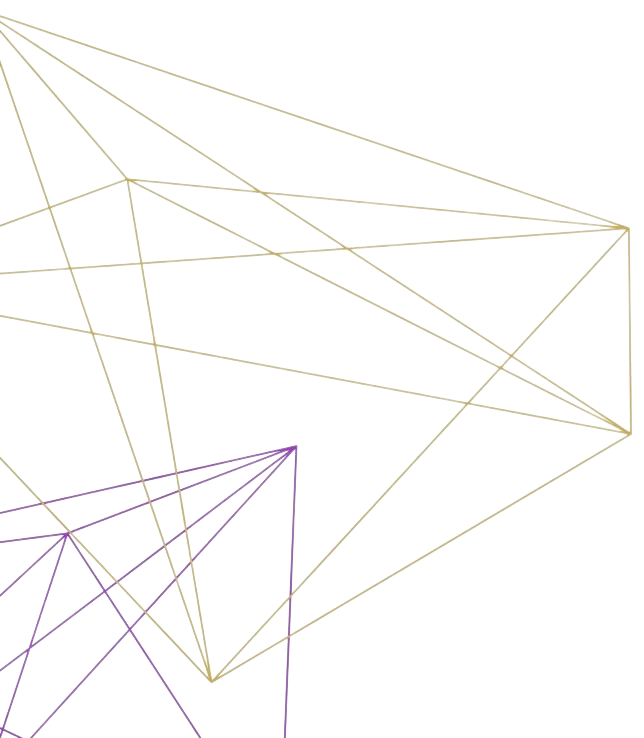
\includegraphics[angle=90,width=0.5\paperwidth,height=0.5\paperheight]{/root/.config/latex-utils/logos/invert2.png}};

\tableofcontents




\newpage

\section{Distributions}

\subsection{Motivation}

When we start with real analysis, we start with functions, limits, and derivatives, and in the end, we will reach differential equations Fourier series and the Fourier transform. The problem begins when we want to look at a solution with sudden changes, such as a sharp term. The notion of the derivative is too strong to consider such a function because, at those sharp points, the solution is not differentiable. We need something new that can then deliver more general solutions.

\begin{example}
    In 1927, Paul Dirac wanted to evaluate the derivative of the Heavyside function $H: \R \longrightarrow \R$, $t \longmapsto 1$ if $t \geq 0$ and $0$ otherwise. This is not a problem for any value different to $0$ but poses a problem at $0$ since there is a discontinuous jump. He then named the delta function $\delta$ the general derivative of the Heavyside function. Thus $\ds{\delta(x)=0}$, $\forall x \neq 0$. \\
    However, he also wanted the fundamental theorem of calculus to hold for the delta function. More concretely, this means that he wanted the following to hold:
    \linecenter{for $\ds{\epsilon>0:\quad \int\limits_{-\epsilon}^{\epsilon} \delta(x) \,d x = \int\limits_{-\epsilon}^{\epsilon} H'(X) \,d x = H(\epsilon)-H(-\epsilon) = 1 -0 = 1}$}
    However nice this may look, the definition of the delta function and the fundamental theorem of calculus are incompatible. The delta function is equal to $0$ everywhere except at one point, which would mean that it is equal to $0$ almost everywhere (with respect to the Lebesgue measure). From this point of view, the integral of the delta function is $0$ and not $1$.

    And because Dirac is an utter buffoon, he also wanted his function to be differentiable, such that $\ds{\delta',\delta'',\delta''',\ldots}$ exist. To place some sense into this lunacy we will define a new object called the distribution, where $\delta$ is an example of such distribution.
\end{example}

For the reasons shown in the example, we will want to calculate with distributions (also called generalized functions). The overall idea is that we view these objects as densities.

\begin{example}
    Visualize a 1-dimensional rod or bar which possesses a mass density, in this picture the delta function represents a single point of mass.

    \begin{minipage}{\textwidth}
        \begin{wrapfigure}{l}{4cm}
            \centering
            \vspace{-0.7cm}
            \begin{tikzpicture}
                \begin{axis}[
                        width=5cm,
                        height=4cm,
                        xtick={10},
                        ytick={10},
                        xmin= -1, xmax= 7,
                        ymin= -0.15, ymax = 0.9,
                        axis lines = middle,
                    ]
                    \draw[red] (axis cs: -1,0.2) .. controls (axis cs: 0,0.5) and (axis cs: 0.5,-0.5) .. (axis cs: 1,0.2) .. controls (axis cs: 1.5,0.9) and (axis cs: 2.5,0.9) .. (axis cs: 3,0.2) .. controls (axis cs: 3.5,-0.5) and (axis cs: 4,0.5) .. (axis cs: 5,0.2) .. controls (axis cs: 6,0.5) and (axis cs: 7,0.2) .. (axis cs: 7,0.2);

                    \draw[blue] (axis cs: 2,0) -- (axis cs: 2,0.7) node [above] {\scriptsize high density};
                    \draw[blue] (axis cs: 5,0) -- (axis cs: 5,0.2) node [above,yshift=4pt] {\scriptsize low density};
                    \draw[green] (axis cs: 1.5,0) .. controls (axis cs: 2,0) and (axis cs: 1.9,0.75) .. (axis cs: 2.25,0.75) .. controls (axis cs: 2.6,0.75) and (axis cs: 2.5,0) .. (axis cs: 3,0) ;
                \end{axis}
            \end{tikzpicture}
        \end{wrapfigure}
        Consider the following mass distribution in red. To find the density of the mass at a point $x$ we would use measurement in real life, but in mathematics, we use "test functions", $\varphi: \R \longrightarrow \R $, which are continuous and localized in some sense.\vspace{10pt}

        If we want to find the mass in that region, we would integrate the integral of the mass distribution and the test function. The result in the mass density in the green region.
        \linecenter{$\ds{\int\limits_{\R}^{} f(x)\varphi(x) \,d x \in \R}$}
    \end{minipage}

    The idea is that we use a lot of these small bumps  such that we can retrieve many real numbers, and generate a map, that maps all the test functions to the real numbers. Instead of looking at $f$ itself, we can look at the collection of all the real numbers that we get from the test functions. This collection is called the distribution of $f$.

    For the delta function, this means that if we measure it using our test function $\varphi$ we would retrieve only $\varphi(0)$.

\end{example}

\subsection{Test functions}

As seen previously, test functions are to be seen as a measurement device, which we use in a very small region. These functions are to be described as infinitely differentiable and compactly supported.

Until now we've only considered functions in the 1-dimensional case, but we can generalize this to the $n$-dimensional case. To do so we define our test functions as $\varphi: \R^n \longrightarrow \R $ (or $\C$). The space of the test function is then defined as $\mathcal{D}(\R^n)$. This space is defined as a space where all test functions are infinitely differentiable $\ds{\mathcal{C}^{\infty}_{c}(\R^n)}$ where $c$ denotes compact support.

The first thing to notice is that $\ds{\mathcal{D}}$ is a vector space, which means that if we choose two functions out of this space, the sum remains differentiable arbitrarily often and vanishes outside a bounded set. That's nice enough but we still want more, we want a specific notion of convergence for this space, which we'll explain later. We can obtain this convergence if we choose a suitable topology or metric, what isn't sufficient is to choose a norm of the vector space, then we won't be able to obtain the desired convergence.

\begin{example}
    Let $\ds{\varphi:\R^n \longrightarrow \R}$ in n-dimentions. The simplest example is a function which is 0 everywhere. But what about other functions?

    We can choose a function that is 0 everywhere except for a certain range such as
    \linecenter{$\ds{\varphi(x)=\exp(-\frac{1}{(1-\| x\|)^2})}$ for $\|x\|<1$ and $0$ otherwise.}
    Indeed the function resembles a bell curve, which is infinitely differentiable and vanishes outside a bounded set.
\end{example}

As a means to define notations, we define the compact support of functions as
\linecenter{$\ds{\operatorname{Supp}(\varphi)=\overline{\left\{ x\in \R^n | \varphi(x)\neq 0 \right\} }}$}
Because we want the closed subset of our function, we take the closure above of the set. If the support is bounded we can add that it is also closed and thus a compact support.

For the notation of partial derivatives, we can use multi-index notations $\ds{\alpha_1,\alpha_2,\ldots,\alpha_n \in \N_0}$, we then call $\ds{\alpha = (\alpha_1,\alpha_2,\ldots,\alpha_n)}$ a multi-index. In this case, $\ds{\alpha_1}$ means that we form the partial derivative with respect to $1$, $\alpha_1$ times. We can then define the partial derivative of a function as:
\linecenter{$\ds{D^\alpha=\frac{\partial^{\alpha_1}}{\partial X_{1}^{\alpha_1} }\frac{\partial^{\alpha_2} }{\partial X_{2}^{\alpha_2}} \ldots \frac{\partial^{\alpha_n} }{\partial X_{n}^{\alpha_n}}}$}

\begin{example}
    $\ds{f: \R^2 \longrightarrow \R}$, $f(x_1,x_2)=2x_{1}^{2}x_{2}^{3}$

    With $\ds{\alpha=(2,1)}$ we can calculate the partial derivative as
    \linecenter{$\ds{(D^\alpha f)(x_1,x_2) = \frac{\partial^2 }{\partial x_{1}^2}\left( \frac{\partial }{\partial x_2} 2x_{1}^{2}x_{2}^{3} \right)  = \frac{\partial^2 }{\partial x_{1}^2}\left( 6x_{1}^{2}x_{2}^{2} \right)  = 12 x_{2}^{2}}$}
\end{example}

This means we can rewrite our $\ds{\mathcal{C}^{\infty}}$ functions. These functions are in $\ds{\mathcal{C}^{\infty}}$ if all the functions $D^\alpha f$ make sense no matter the multi-index $\alpha$. Putting this into notation :
\linecenter{$\ds{\varphi \in \mathcal{C}^{\infty} \iff \forall \alpha \in \N_0^n: D^\alpha f \in \mathcal{C}(\R^n)}$}
With this knowledge, we can form more test functions and explain what the special convergence from above means.

\subsection{Convergence of test functions}

Recall that the set of test functions is denoted by $\ds{\mathcal{D}(\R^n)=\mathcal{C}^{\infty}_{c}}$ which also forms a vector space. In this vector spaces setting, if we have a norm in such a vector space, we can say that a sequence of function convergence to another function if the norm of the difference between the two functions converges to $0$, justified by using the norm $\ds{\|\cdot \|}$.
\linecenter{$\ds{f_n \longrightarrow f \iff \|f_n-f\| \overset{n\to \infty}{\longrightarrow} 0}$}
If we have a metric we can also say $\ds{f_n }$ converges to $\ds{f }$ if the distance measured in the metric goes to $\ds{0}$ when $n$ goes to $\ds{\infty}$.
\linecenter{$\ds{f_n \longrightarrow f \iff d(f_n,f)\overset{n\to \infty}{\longrightarrow}0}$}
But both notions are not sufficient in our context, for this we need a very strong notion of convergence. We need to define a convergence where differentiability and compact support are kept.



\begin{minipage}{\textwidth}
    \begin{wrapfigure}{r}{5cm}
        \begin{tikzpicture}
            \begin{axis}[
                    width=5cm,
                    height=4cm,
                    xtick={10},
                    ytick={10},
                    xmin= -1, xmax= 7,
                    ymin= -0.15, ymax = 0.9,
                    axis lines = middle,
                ]
                \draw[green] (axis cs: 1.5,0) .. controls (axis cs: 2,0) and (axis cs: 1.9,0.2) .. (axis cs: 2.25,0.2) .. controls (axis cs: 2.6,0.2) and (axis cs: 2.5,0) .. (axis cs: 3,0) ;
                \draw[blue] (axis cs: 0.5,0) .. controls (axis cs: 1.5,0) and (axis cs: 1.9,0.5) .. (axis cs: 2.25,0.5) .. controls (axis cs: 2.6,0.5) and (axis cs: 3,0) .. (axis cs: 4,0) ;
                \draw[red] (axis cs: -0.5,0) .. controls (axis cs: 1,0) and (axis cs: 1.9,0.8) .. (axis cs: 2.25,0.8) .. controls (axis cs: 2.6,0.8) and (axis cs: 3.5,0) .. (axis cs: 5,0);

                \node[above,color=green] at (2.25,0.2) {\scriptsize $\varphi_1$};
                \node[above,color=blue] at (2.25,0.5) {\scriptsize $\varphi_2$};
                \node[above,color=red] at (3,0.7) {\scriptsize $\varphi_3$};

            \end{axis}
        \end{tikzpicture}
    \end{wrapfigure}
    We define this as follows: for any sequence of test function $\ds{(\varphi_k)_{k \in  \N}\subset \mathcal{D}(\R^n)}$, and test function $\ds{\varphi \in \mathcal{D}(\R^n)}$ we write the new convergence of test functions as $\varphi_k \underset{\mathcal{D}}{\longrightarrow} \varphi$ if all the functions in the sequence live on the same compact set. In other words, what we want to avoid is having our test functions get larger and larger, such that the limit would no longer be a test function.
\end{minipage}

This coincides with the notion that a test function should always test the bounded set, which is something we want to conserve in our convergence. Therefore we specify that there should be a bounded set $M$ such that outside of this set, $\ds{\varphi_k=0}, \forall k$. This means that all the information of all the functions lies in the set $M$.



\begin{minipage}{\textwidth}
    \begin{wrapfigure}{r}{5cm}
        \begin{tikzpicture}
            \begin{axis}[
                    width=5cm,
                    height=4cm,
                    xtick={10},
                    ytick={10},
                    xmin= -1, xmax= 7,
                    ymin= -0.15, ymax = 0.9,
                    axis lines = middle,
                ]

                \draw[blue] (axis cs: 0.5,0) .. controls (axis cs: 1.5,0) and (axis cs: 1.9,0.5) .. (axis cs: 2.25,0.5) .. controls (axis cs: 2.6,0.5) and (axis cs: 3,0) .. (axis cs: 4,0) ;
                \draw[blue,dashed](axis cs: -1,-0.145)-- (axis cs: 0.5,-0.145) .. controls (axis cs: 1.5,-0.145) and (axis cs: 1.9,0.35) .. (axis cs: 2.25,0.35) .. controls (axis cs: 2.6,0.35) and (axis cs: 3,-0.145) .. (axis cs: 4,-0.145) -- (axis cs: 7,-0.145);
                \draw[blue,dashed](axis cs: -1,0.15)-- (axis cs: 0.5,0.15) .. controls (axis cs: 1.5,0.15) and (axis cs: 1.9,0.65) .. (axis cs: 2.25,0.65) .. controls (axis cs: 2.6,0.65) and (axis cs: 3,0.15) .. (axis cs: 4,0.15) -- (axis cs: 7,0.15);


                \node[above,color=blue] at (3,0.5) {\scriptsize $\varphi$};
            \end{axis}
        \end{tikzpicture}
    \end{wrapfigure}
    Another condition that needs to be satisfied is that of uniform convergence, such that the sequence of functions $\ds{\varphi_k}$ should converge uniformly to $\ds{\varphi}$, $\ds{\varphi_k \underset{\text{unif}}{\longrightarrow} \varphi}$.

    Almost all of the functions of the sequence $\ds{\varphi_k}$ lie inside the tube seen in the graph. This is what is called uniform convergence because the convergence works for all points in the domain simultaneously, therefore it is stronger than point-wise convergence where only one point is considered at a time.
\end{minipage}
Now to satisfy our needs for differentiation we also need the derivatives of our test functions to also converge uniformly. Which means that $\ds{\forall \alpha, D^\alpha \varphi_k  \underset{\text{unif}}{\longrightarrow} D^\alpha \varphi }$.

Both of these conditions can be put in a short form using the supremum norm defined for functions as $\ds{\|f\|_{\infty}=\sup_{x \in \R^n} |f(x)|}$ which is the maximum value the function can reach.

The uniform convergence is exactly the convergence with respect to the supremum norm. Hence we can then write the following :
\begin{theorem}
    For any sequence of test functions $\ds{(\varphi_k)_{k \in  \N}\subset \mathcal{D}(\R^n)}$, and test function $\ds{\varphi \in \mathcal{D}(\R^n)}$, then the convergence is defined as:
    \linecenter{$\ds{\varphi_k \underset{\mathcal{D}}{\longrightarrow} \varphi \iff \exists C \underline{\subset } \R^n }$ a compact support such that $\ds{\operatorname{Supp}(\varphi_1),\operatorname{Supp}(\varphi_2),\ldots \underline{\subset } C}$ }
    \linecenter{and $\ds{\forall \alpha}$ we have $\ds{\|D^\alpha \varphi_k - D^\alpha \varphi\| \overset{k\to \infty}{\longrightarrow}0 }$}
\end{theorem}

\subsection{Definition of distributions}

Here will define the notion of distributions. At this point, we have introduced the space of test functions $\ds{\mathcal{D}(\R^n)}$ and the notion of convergence for sequences of test functions $\ds{\varphi_k \underset{\mathcal{D}}{\longrightarrow} \varphi}$, which is a special case of topological vector spaces.

A distribution is denoted by $\ds{T:\mathcal{D}(\R^n)\longrightarrow\R}$, this should be a map for the test function into the real or complex numbers depending on whether we are looking at real or complex functions. What should then be remembered is that distribution takes a function as input and always returns a number as output.

However this definition is not sufficient, we want $\ds{T}$ to be linear  such that $\ds{T(\varphi_1+\varphi_2)=T(\varphi_1)+T\varphi_2}$ and $\ds{T(\lambda\varphi)=\lambda\cdot T(\varphi)}$. The second property refers to the notion of convergence, which means that $\ds{T}$ should be continuous. Using the notion of convergence for sequences of test functions we can relate to the continuity of $\ds{T}$ by looking at how it is sequentially convergent.


\begin{theorem}
    For all $\ds{\varphi\in \mathcal{D}(\R^n)}$ and for all sequences $\ds{(\varphi_k)_{k\in \N}\underline{\subset }\mathcal{D}(\R^n)}$ with $\ds{\varphi_k\underset{\mathcal{D}}{\longrightarrow}\varphi}$ :\\
    A distribution $\ds{T:\mathcal{D}(\R^n)\longrightarrow\R}$ is continuous if and only if $\ds{\varphi_k \underset{\mathcal{D}}{\longrightarrow} \varphi}$ implies $\ds{T(\varphi_k) \overset{k\to \infty}{\longrightarrow} T(\varphi)}$.
\end{theorem}

For these distribution, the space of distributions is denoted by $\ds{\mathcal{D}'(\R^n)}$.

\begin{example}
    Consider the delta distribution: $\ds{\delta:\mathcal{D}(\R^n)\longrightarrow\R}, \varphi \longmapsto \varphi(0)$.

    This is a linear map because $\ds{\delta(\varphi_1+\varphi_2)=(\varphi_1+\varphi_2)(0)=\varphi_1(0)+\varphi_2(0)=\delta(\varphi_1)+\delta(\varphi_2)}$ and $\ds{\delta(\lambda\varphi)=(\lambda\varphi)(0)=\lambda\varphi(0)=\lambda\delta(\varphi)}$.

    We can also show that $\ds{\delta}$ is continuous. Let $\ds{\varphi_k \underset{\mathcal{D}}{\longrightarrow} \varphi}$, then $\ds{\varphi_k(0) \overset{k\to \infty}{\longrightarrow} \varphi(0)}$ because $\ds{\varphi_k}$ converges uniformly to $\ds{\varphi}$, which means that $\ds{\varphi_k(0)}$ converges to $\ds{\varphi(0)=\delta(\varphi)}$.

\end{example}

\end{document}